%% LyX 2.1.2 created this file.  For more info, see http://www.lyx.org/.
%% Do not edit unless you really know what you are doing.
\documentclass[10pt]{article}
\usepackage[T1]{fontenc}
\usepackage[utf8x]{inputenc}
\usepackage{geometry}
\geometry{verbose,tmargin=2.5cm,bmargin=2.5cm,lmargin=2cm,rmargin=1.5cm,headsep=0.5cm,footskip=1cm}
\setcounter{secnumdepth}{3}
\setcounter{tocdepth}{3}
\usepackage{color}
\usepackage{amsthm}
\usepackage{amsmath}
\usepackage{amssymb}
\usepackage{graphicx}
\usepackage{setspace}
\doublespacing
\usepackage[unicode=true,pdfusetitle,
 bookmarks=true,bookmarksnumbered=true,bookmarksopen=true,bookmarksopenlevel=1,
 breaklinks=false,pdfborder={0 0 1},backref=section,colorlinks=true]
 {hyperref}
\hypersetup{
 urlcolor=blue,citecolor=blue}

\makeatletter

%%%%%%%%%%%%%%%%%%%%%%%%%%%%%% LyX specific LaTeX commands.
%% Because html converters don't know tabularnewline
\providecommand{\tabularnewline}{\\}

%%%%%%%%%%%%%%%%%%%%%%%%%%%%%% Textclass specific LaTeX commands.
  \theoremstyle{definition}
  \newtheorem{defn}{\protect\definitionname}
  \theoremstyle{plain}
  \newtheorem{prop}{\protect\propositionname}

%%%%%%%%%%%%%%%%%%%%%%%%%%%%%% User specified LaTeX commands.
\@ifundefined{definecolor}
 {\usepackage{color}}{}
\@ifundefined{definecolor}{\usepackage{color}}{}
\@ifundefined{definecolor}{\usepackage{color}}{}
\@ifundefined{definecolor}{\usepackage{color}}{}
\@ifundefined{definecolor}{\usepackage{color}}{}
\@ifundefined{definecolor}{\usepackage{color}}{}
\@ifundefined{definecolor}{\usepackage{color}}{}
\@ifundefined{definecolor}{\usepackage{color}}{}
\@ifundefined{definecolor}{\usepackage{color}}{}
\@ifundefined{definecolor}{\usepackage{color}}{}
\@ifundefined{definecolor}{\usepackage{color}}{}

%\usepackage[french]{babel}
\usepackage{booktabs}\usepackage[format=plain,labelsep=endash,labelfont=bf]{caption}


 %\linenumbers

\makeatother

  \providecommand{\definitionname}{Definition}
  \providecommand{\propositionname}{Proposition}

\begin{document}

\title{Reference Document for Giang's Ph.D. Subject}


\date{16/04/2015 Version 1.1}


\title{Quantifying the effect of synchrony on the persistence of infectious
diseases in a metapopulation}


\author{Tran Thi Cam Giang, Marc Choisy, Jean-Daniel Zucker, Yann Chevaleyre}
\maketitle
\begin{abstract}
Global persistence of infectious diseases is a big problem for epidemiologists.
Studies have showed that there are a lot of reasons to answer why
many communicable diseases still exist and have been developed in
more dangerous form \cite{binder1999emerging,jones2008global,morens2004challenge,patz1996global,tenover1996challenges}.
The asynchrony and the recolonization among subpopulations are two
key reasons pointed out. However, why these are the asynchrony and
the recolonozations in a metapopulation is still an open question.
Here we study the combined effects of forcing phase heterogeneity
in the seasonally forced contact rate on global persistence of disease.
We carry out an exploitation of stochastic dynamics in a susceptible-exposed-infectious-recovered
(SEIR) model of the spread of infectious diseases in a metapopulation
of n subpopulations. Starting with continuous-time Markov description
of the model of deterministic equation, the direct method of Gillespie(1977)
\cite{gillespie1977exact} in the class of Monte-Carlo simulation
methods allows us to simulate exactly the spread of disease with the
SEIR model. Our finding of the exploitation of stochastic dynamics
points out that the persistence of the disease in the meta-population
is characterized as an exponential survival model on data simulated
by the stochastic model. Using a parametric survival model for an
exponential distribution (R package 'survival' \cite{survival-package}),
we estimate the global extinction rate which represents the global
persistence of disease in the meta-population. We find how bigger
the forcing phase heterogeneity becomes, and how larger the global
persistence gets.

\textbf{Keywords}: SEIR model, Markov chain, Monte-Carlo simulation
methods, spatial synchronization, disease persistence, meta-population. 
\end{abstract}

\section{INTRODUCTION}

News about infectious diseases has always been a subject of worry
to parents as well as all. It has brought many problems to humain
society. Recent works have shown that infectious diseases do spread
in space \cite{Cumming2004,Grenfell2001,Smith2004,viboud2006synchrony}.
The exact form of disease movement depends on a number of local factors
(demographic including population size \cite{Hagenaars2004}, growth
rate and death rate \cite{Conlan2007}, sociological such as school
period of children, work tendency from rural to urban, environmental
and climatic comprising seasonal variations in seasonality \cite{Conlan2010,Griffen2009},
temperature and rainfall, immunological for diseases, etc...) as well
as the connections between the different populations (i.e. spatial
structure) \cite{Yan2007} such as distance \cite{Hagenaars2004},
coupling rate, number of individuals between populations, etc....Hence,
we focus on spread of disease in space by using variations in the
seasonal aspects of subpopulations and after examine how synchrony
could affect the persistence of infectious diseases in a metapopulation.

In modeling of ecological system, presenting interactions between
humans, subpopulations, geographic conditions and the metapopulation
model is a good choice. Metapopulation is a set of subpopulations
with mutual interaction \cite{Levins1969} here a subpopulation can
only go extinct locally and be recolonized by another after it is
emptied by extinction \cite{Bolker1996,Hanski1998,Levins1969}. It
is the reason that the ecological theory of metapopualtion can point
out that the persistence of a population depends on the dynamics of
migrations between the different sub-populations of the metapopualtion
\cite{Hagenaars2004,Hanski1998,Hanski2004,Levins1969}. The “colonization”
caused by migrations brings infection to an uninfected subpopulation
and we call infected individuals colonizers.

In addition, the disease persistence capability in a metapopulation
depends positively on level of asynchrony between subpopulations \cite{Hagenaars2004,Heino1997}.
Many studies showed that the asynchronization of epidemics among subpopulations
causes the recolonization of diseases for locally extinct subpopulation
\cite{Bolker1996,Hagenaars2004,Hanski1998,Heino1997,Yaari2012}. So,
the recolonization becomes the main reason for which disease persistence
exists. The disease always appears in metapopulation if and only if
there is at least one non-extinct subpopulation.\textbf{ }In 1996\textbf{,
}in order to explain why measles persists after lot of vaccination
policies, Bolker \cite{Bolker1996} used the measles data before and
after vaccination from 1964 to 1988 in England and Wales. Vaccination
has broken high synchrony between the UK cities in prevaccination
era, and at the same time, causes decorrelation and enhances global
persistence of the infection, because of decorrelating factors of
vaccination such as the starting moment of vaccination policies, number
of susceptibles vaccinated and interaction between vaccination policies
\cite{Bolker1996,Rohani1999}. A decrease in correlation between subpopulations
may make a metapopulation more difficult to eradicate infectious diseases\textbf{
}\cite{Bolker1996,Earn1998}. In addition, the level of synchrony
between the subpopulations is strongly governed by the migration rate
and distances between them \cite{Heino1997}. In our modern world,
the distance problem isn't large anymore for individuals who want
to travel. There are a lot of cities very remote, but very connected,
and thus very synchronous as in the USA \cite{Choisy2012}. In contrast,
migration among subpopulations has become a big problem. The disease
synchrony speed within a metapopulation can strongly increase when
migration rate there is strong \cite{KeelingRohani2008}.\textbf{
}The migration rates are directly proportional to the amount of variation
in metapopulation size, but inversely to the amount of variation in
subpopulation size, over time \cite{Dey2006,Griffen2009}. So, migration
is key to the recolonization of empty subpopulation and simultaneously
increases the degree of synchrony between subpopulations in spatially
structured metapopulation. However, the vast majority of infectious
diseases control policies that are applied in the world are still
based on rationales that do not consider the local extinction/recolonization
dynamics. This is maybe a reason why measles persists\textbf{ }around
the world, despite highly local vaccine coverages \cite{Conlan2007}.
For example, in the start of the 2014, the World Health Organization
(WHO) had officially stated the global measles epidemic outbreak.
In the first three months of the year 2014, there were about 56,000
cases of measle infections in 75 countries \cite{WHO2014a}, including
countries in south-east Asia and most particularly, Vietnam \cite{http://healthmap.org/site/diseasedaily/article/measles-reemerges-vietnam-22814}.
We discovered measles persistence in the world for many years without
extinction, from one nation to another as well as from cities to other
cities. Though the moment of disease outbreaks in each region differs.
For neighbouring regions with disease persistence, there is a time-lag
differs between disease outbreak. This is explained in sociology by
difference in culture, in geographic condition and more particularly
seasonality.

Seasonality has been one in rather robust ingredients influencing
the disease persistence process. Seasonal changes can alter migration
tendency between urban and rural areas \cite{Ferrari2010}, also residence
time of hosts, vectors and pathogens. Seasonal variation can thus
determine population size, migration and interaction capabilities
and particularly infection rate at which susceptible individuals become
infected \cite{Altizer2006,Hosseini2004}. Hence, infectious disease
outbreak occurs due to this infection rate. However, finding a clear
mechanism of seasonal forcing for modelling is a very difficult work
because of unidentified formula for seasonal forcing \cite{Altizer2006,Ferrari2010}.
For indirectly transmission diseases such as water-born and vector-born,
finding seasonality characteristics is less a problem, however, in
direct contrast to transmission diseases such as measles. Seasonal
forcing in a metapopulation is influenced by weather and climate in
region, school schedule of children, and rural-urban migration in
countries \cite{Bolker1995,Conlan2007,Ferrari2010,Gunning2013}. In
these factors, the seasonal aggregation of children in primary schools
affects clearly the infection rate in metapopulation. The infection
rate decreases due to children holidays but is inverse when the children
come back to school \cite{Conlan2007}.\textbf{ }So\textbf{, }exploring
the influence of seasonality for the infection rate in simulation
has been developed in many previous years. If the infection rates
given are the same in all subpopulations, so this metapopualtion model
is a rather simple model \cite{Rozhnova2012,Rozhnova12013} and the
symmetry of the fixed points among subpopulations will not be broken.
In contrast, if the infection rate is different in all subpopulations,
so we have a more complex oscilation metapopulation model, but close
to the oscilations in reality. Thus, realizing the oscilations of
infectious diseases in life within metapopulation simulation models
to estimate global disease persistence time has become a large problem
and the infectious disease eradication has become our aim\textbf{
}\cite{Earn1998}.

Here we propose a simulation study to quantify the effect of synchrony
on the persistence of infectious diseases. We use stochastic simulations
for infectious diseases in a metapopualtion, then we consider different
spatial structures from the simplest to complex. These forcings can
reflect local demographic, sociological, environmental, or climatic
factors. The level of synchrony is computed from the phases of forcing
in the different subpopulations and persistence is quantified by using
statistical tools from survival analysis. Here, we are concerned about
measles and simultaneously use the parameter values from articles
and measles reports. As the persistence of measles has been largely
studied in the literature and its still unexplained while global persistence
is a growing concern for WHO and public health authorities around
the world \cite{Conlan2010}.

To do this, we first build the deterministic model for a metapopualtion.
Then, we describe the spatial structure and the stochastic version
of the model. Finally, we introduce the characterization of global
persistence in the metapopulation based on the measles characteristics.


\section{MATERIAL AND METHODS }


\subsection{MATERIAL}


\subsubsection{Deterministic model for many subpopulations}

The standard SEIR model (susceptible-exposed-infective-recovered)
has been strongly developed for the dynamics of directly infectious
disease \cite{Bolker1995}. For disease-based metapopulation models,
we give here a suitable new version of the SEIR equation that would
be as follows:

Consider a metapopulation of $n$ sub-populations. In a subpopulation
$i$ of size $N_{i}$, disease dynamics can be deterministically described
by the following set of differential equations \cite{Anderson&May1992}:

\begin{eqnarray}
\frac{dS_{i}}{dt} & = & \mu N_{i}-\lambda_{i}S_{i}-\mu S_{i}\label{eq:dS}\\
\frac{dE_{i}}{dt} & = & \lambda_{i}S_{i}-\mu E_{i}-\sigma E_{i}\\
\frac{dI_{i}}{dt} & = & \sigma E_{i}-\mu I_{i}-\gamma I_{i}\label{eq:infectieux}\\
\frac{dR_{i}}{dt} & = & \gamma I_{i}-\mu R_{i}\label{eq:dR}
\end{eqnarray}
 where $S_{i}$, $E_{i}$, $I_{i}$ et $R_{i}$ are the numbers of
susceptible, exposed, infectious and recovered in this sub-population
$i$ respectively. Individuals are born susceptible, die at a rate
$\mu$, become infected with the force of infection $\lambda_{i}$,
infectious after a latency period of an average duration of $1/\sigma$
and recover at the rate $\gamma$. In a case the infectious contact
rate is constant, the equilibrium values of the variables $S$, $E$,
$I$ and $R$ can be expressed analytically (see appendix). The force
of infection depends not only on the total population size $N_{i}$
and the number of infected $I_{i}$ in subpopulation $i$, but also
in other sub-populations\textbf{ \cite{KeelingRohani2008} :}

\textbf{
\begin{equation}
\lambda_{i}=\sum_{j}\rho_{ij}\kappa_{j}\log\left[1-\sum_{k=1}^{M}\left(\frac{\left|I_{k,t}\right|}{N_{k}}\times c_{ik}\times\xi_{jk}\right)\right]\label{eq:force-1}
\end{equation}
 }where\textbf{ }$c_{i,k}$ ($0\leqslant c_{ij}\leqslant1$) is the
probability that a susceptible individual native from $i$ being in
contact with another infected individual native from $k$ gets infected.
$\xi_{jk}$ ($0\leqslant\xi_{ij}\leqslant1$) refers to the probability
that an individual $y$ meeting $x$ in $C_{j}$ comes from $C_{k}$.\textbf{
}$\kappa_{j}$ is the average number of contacts per unit of time
a susceptible will have when visiting subpopulation $j$. $\rho_{i,j}$
($0\leqslant\rho_{ij}\leqslant1$) is denoted as the probability that
an individual from subpopulation $i$ visits subpopulation $j$, of
course, $\sum_{j=1}^{M}\rho_{ij}=1$. See appendix for detail on the
construction of this equation. We can verify that in the limit case
on one single subpopulation in the metapopulation ($i=j$ and $n=1$)
we have 
\begin{equation}
\lambda_{i}=-\kappa_{i}\log(1-\frac{I_{i}}{N_{i}}\times c_{ii})
\end{equation}
 Consider that the average number of contacts per unit of time $\kappa_{i}$
is seasonally forced \cite{Altizer2006} and seasonality is an annually
periodic function of time \cite{Grenfell1995}. As a result, for the
subpopulation $i$ : 
\begin{equation}
\kappa_{i}(t)=\kappa_{i0}\left[1+\kappa_{i1}\cos\left(\frac{2\pi t}{T}+\varphi_{i}\right)\right]\label{eq:beta_i}
\end{equation}
 where $t$ is the time, $\kappa_{i0}$ and $\kappa_{i1}$ are the
mean value and amplitude of the average contact rate $\kappa_{i}$
at which a susceptible will have when visiting subpopulation $i$
per unit of time, $T$ and $\varphi_{i}$ are the period and the phase
of the forcing. With the annual sinusoidal form of the average contact
rate, we really have the sinusoidally forced SEIR metapopulation model.


\subsubsection{Stochastic model for many subpopulations}

In order to study the persistence of the disease, we must consider
a stochastic version of the model \cite{Keeling2002,Lloyd2001,renshaw1993modelling}.
We use for that a population-based time-to-next-event model based
on Gillespie's algorithm \cite{gillespie1977exact}. Table \ref{tab:stoch_ev}
lists all the events of the model, occurring in subpopulation $i$.

\begin{table}[tbph]
\begin{centering}
\protect\caption{\label{tab:stoch_ev}Events of the stochastic version of the model
of equations \ref{eq:dS}-\ref{eq:dR}, occuring in subpopulation
$i$.}

\par\end{centering}

\centering{}%
\begin{tabular}{lcc}
\toprule Events  & Rates  & Transitions \tabularnewline
\midrule birth  & $\mu N_{i}$  & $S_{i}\leftarrow S_{i}+1$ and $N_{i}\leftarrow N_{i}+1$ \tabularnewline
death of a susceptible  & $\mu S_{i}$  & $S_{i}\leftarrow S_{i}-1$ \tabularnewline
death of an exposed  & $\mu E_{i}$  & $E_{i}\leftarrow E_{i}-1$ \tabularnewline
death of an infected  & $\mu I_{i}$  & $I_{i}\leftarrow I_{i}-1$ \tabularnewline
death of an immune  & $\mu R_{i}$  & $I_{i}\leftarrow I_{i}-1$ \tabularnewline
infection  & $\lambda_{i}S_{i}$  & $S_{i}\leftarrow S_{i}-1$ and $E_{i}\leftarrow E_{i}+1$ \tabularnewline
becoming infectious  & $\sigma E_{i}$  & $E_{i}\leftarrow E_{i}-1$ and $I_{i}\leftarrow I_{i}+1$ \tabularnewline
recovery  & $\gamma I_{i}$  & $I_{i}\leftarrow I_{i}-1$ and $R_{i}\leftarrow R_{i}+1$ \tabularnewline
\bottomrule  &  & \tabularnewline
\end{tabular}
\end{table}



\subsubsection{Spatial structures}

A metapopulation is a population of populations (subpopulations).
Such a structure implies an heterogeneity in the sense where the probability
of contact (or contact rate) between individuals from a same subpopulation
is higher than the probability of contact between individuals of different
subpopulations \cite{Hanski2004}. Such heterogeneity is actually
the result of the interaction between two phenomena that are often
difficult to disentangle in nature. The first one relates to the granularity
of the metapopulation (as rendered by the number of and sizes of subpopulations)
and the second one relates to the isolation between subpopulations
(as can be rendered, among others, by physical distances separating
each pair of subpopulations). Moreover, according to the findings
of Benjamin Bolker (1995) \cite{Bolker1995}, there is no coexistence
between periodicity and disease persistence in non-spatial measles
models, and spatial structure is an important factor to both enhance
persistence and create new types of dynamic behaviour.

To identify clearly the causes of observed phenomena, these two aspects
will be modeled distinctly. In this article, our null model (model
0) will be a metapopulation without any explicit spatial distance
(all the subpopulations are at the same distance from each other)
and where all the metapopulation have the same population size $N$.
Like the original Levins's model \cite{Levins1969}, this model considers
that all the subpopulations are at equal distance from each other:
\begin{equation}
\rho_{ij}=\rho,\qquad0\leqslant\rho\leqslant1,\qquad\forall i,\forall j.
\end{equation}
 The structure of this metapopulation is thus characterized by 3 parameters:
(i) the number $n$ of sub-populations, (ii) the population size $N$
($N_{i}=N$, $\forall i$) of all these subpopulations and, (iii)
the coupling (or distance) $\rho_{ij}$ between two subpopulations
$i$ and $j$ that refers to the the probability that an individual
from subpopulation $i$ visits subpopulation $j$.


\subsection{METHOD}


\subsubsection{Stationary distribution in metapopulation}

Here we show some assumptions for the stationary distribution model
as follows :
\begin{itemize}
\item Assumption 1. For each subpopulation $V_{i}$, there exists a markov
chain $M_{i}$ describing where (i.e. in which subpopulation) individuals
native from $V_{i}$ travel at each time step. 
\item Assumption 2. Each $M_{i}$ has a stationary distribution $\rho(M_{i})$. 
\item Assumption 3. At time t=0, each agent is located in a subpopulation
randomly drawn from $\rho(M_{i})$.
\end{itemize}
Therefore, when we consider a simplified model in which the dynamics
of the agents is stationary: each agent native from $V_{i}$ no more
follows a markov chain, but is relocated at each time step on a subpopulation
randomly drawn from $\rho(M_{i})$.

Then, under assumptions 1,2,3, at any time $t$, when the total number
of agents grows to infinity, the size of the populations under the
markovian dynamics converges towards the size of the populations under
stationary dynamics.

Thus, any statistics computed on the densities of agents from the
same population in various cities will not distinguish the markovian
from the stationary dynamics. 

Based on this conclusion, we will deploy a stationary distribution
in a metapopulation by building a transition matrix and then computing
its convergence. This matrix converges towards a stationary distribution
matrix. Finally, we will apply the stationary distribution matrix
in the metapopulation of $n$ subpopulations.


\subsubsection{Global persistence in a metapopulation}

In order to examine questions of interaction between disease transmissibility
and phase of seasonal forcing, we start in this section by studing
the stochastic SEIR model in a metapopualtion of $n$ subpopulations.
For this meta-population, we observe the disease extinction in time
due to spatial synchrony/asynchrony that are influenced by phase difference
in seasonal forcing. To create the phase difference, we change the
value of the forcing phase for each subpopulation. In this experience,
we use a parameter $\varphi_{max}$ in radian that runs in the interval
from zero to $\pi$. With each value of $\varphi_{max}$, based on
$n$ the number of subpopulations in the metapopulation, we divide
the interval $[0,\varphi_{max}]$ into a set of $(n-1)$ equal samples,
so the value of the forcing phase of the $i^{th}$ subpopulation is
correspondent to $i^{th}$ value in the set. We call $\varphi_{max}$
asynchrony parameter.

The persistence of disease in the metapopulation was characterized
by fitting an exponential survival model \cite{Conlan2010,Kleinbaum2005}
on a data simulated by a stochastic model. To measure the persistence
in ecology and epidemiology, so many methods we can use \cite{Conlan2010,Gunning2013,Keeling2002}.
For example, Keeling et al.(2002) \cite{Keeling2002} gave two methods.
One method was for an isolated metapopulation without migration by
calculating the expected extinction time or the extinction rate during
a given period. This was a theoretical measure as no real data exists
to compare with model results. The other method for a population with
migration was found by calculating the number or the total duration
of extinctions. Then in 2010, ``mean annual fade-out'' and ``fade-outs
post epidemic'' methods proposed by Conlan \cite{Conlan2010} were
used to quantify persistence by basing on the proportion or on the
frequency of zero reports in a given reporting interval. In this work,
we propose a new rate that presents also the survival of disease in
a metapopulation. This is the mass extinction rate. For our metapopulation
of $n$ subpopulations, to do so we run first $m$ independent simulations
of our stochastic model. We calculate then the average metapopulation
size by summing subpopulations at each sample time and averaging across
the entire time series for each metapopulation. Lastly, we record
the dates $t$ of global disease extinction in all these $m$ metapopulations.
These dates allow to draw Kaplan-Meier survival curves from which
we estimate the global extinction rates $\chi$: 
\begin{equation}
M(t)=\exp(-\chi t)
\end{equation}
 where $M(t)$ ($0\leqslant M(t)\leqslant m$) is the number of metapopulations
in which the disease is not extinct at time $t$.

We use the parametric survival model for the exponential distribution
(R package '$survival$' \cite{survival-package}) to estimate the
mass extinction rate of a metapopulation during 100 years. Due to
that, we can capture one of the most important features of stochastic
systems in spatial structure : its global extinction characteristics
of disease.

\bigskip{}



\subsubsection{Characterization of synchrony}

Call $\delta_{ij}=\delta_{ji}$ ($0\leqslant\delta_{ij}<2\pi$) the
phase difference between subpopulations $i$ and $j$ : 
\begin{equation}
\delta_{ij}=|\varphi_{i}-\varphi_{j}|\bmod2\pi
\end{equation}
 where $\varphi{}_{i}$ and $\varphi{}_{j}$ are the phases of the
contact rates (equation \ref{eq:beta_i}) in subpopulations $i$ et
$j$. Populations $i$ and $j$ are perfectly in phase if $\delta_{ij}=\delta_{ji}=0$
or $2\pi$ and in opposition of phase if $\delta_{ij}=\delta_{ji}=\pi$.
We can thus define the degree of synchrony $\xi_{ij}=\xi_{ji}$ ($0\leqslant\xi_{ij}\leqslant1$)
between populations $i$ and $j$ as 
\begin{equation}
\xi_{ij}=\left|1-\frac{\delta_{ij}}{\pi}\right|.
\end{equation}
 
\begin{figure}[htpb]
\centering 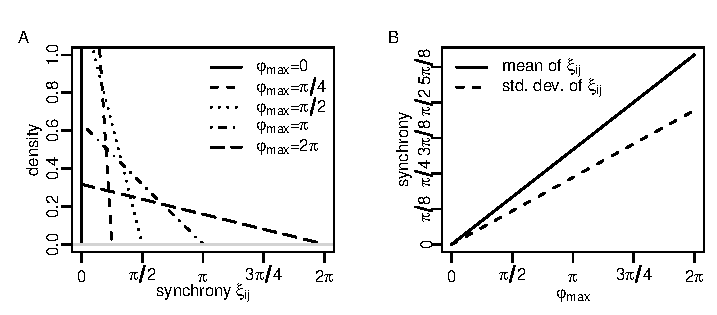
\includegraphics{figure1} \protect\caption{\label{fig:synchrony-1}Synchrony in the case of model 0. (A) distribution
of synchrony $\xi_{ij}$ for various values of $\varphi_{max}$. (B)
mean and standard deviation of the distribution of $\xi_{ij}$ as
functions of $\varphi_{\mbox{\tiny max}}$.}
\end{figure}


Consider that in the metapopulation the phases $\varphi_{i}$ of the
contact rates in the $n$ subpopulations are evenly distributed between
0 and $\varphi_{\mbox{\tiny max}}$ ($0\leqslant\varphi_{\mbox{\tiny max}}\leqslant\pi$).
We can express the mean of the pairwise phase differences $\delta_{ij}=\delta_{ji}$
as 
\begin{equation}
<\!\!\delta_{ij}\!\!>\;=\;<\!\!\delta_{ji}\!\!>\;=2\varphi_{\mbox{\tiny max}}\sum_{k=1}^{n-1}\frac{(n-k)k}{(n-1)n^{2}}=\frac{n+1}{3n}\varphi_{\mbox{\tiny max}}
\end{equation}
 and thus the mean of the synchronies $\xi_{ij}=\xi_{ji}$ as 
\begin{equation}
<\!\!\xi_{ij}\!\!>\;=\;<\!\!\xi_{ji}\!\!>\;=1-\frac{n+1}{3n}\frac{\varphi_{\mbox{\tiny max}}}{\pi}
\end{equation}
 and thus 
\begin{equation}
\lim_{n\to\infty}<\!\!\xi_{ij}\!\!>\;=1-\frac{\varphi_{\mbox{\tiny max}}}{3\pi}
\end{equation}


As illustrated in Figure \ref{fig:synchrony-1}, for a high enough
number $n$ of subpopulations, the mean value of the $\xi_{ij}$ does
not depend on the number of subpopulation.

The values of $\varphi_{i}$ are chosen so that they are uniformly
distributed between $\varphi_{\mbox{\tiny min}}=0$ and $\varphi_{\mbox{\tiny max}}$.
The distribution of $\xi_{ij}$ doesn't depend on $n$ the number
of subpopulation, but only depends $\varphi_{\mbox{\tiny max}}$ and
may be is characterized by one single parameter (we choose the average
value of all $\xi_{ij}$)\textbf{, }view figure \ref{fig:synchrony-1}.


\subsection{Plan of experience}

In this section, we will describe our plan of experience to quantifying
the effect of synchrony on the persistence of infectious diseases
in a metapopulation. We have four big concerns that we must verify.


\subsubsection{Quantifying disease persistence in the simplest metapopulation }

Firstly, we are interested in the correlation between global disease
persistence time and recolonization in metapopulation when the forcing
phase of the average contact rate $\kappa$ in each subpopulation
alters. In order to simplify this concern, we start with the metapopulation
of two subpopulations. To have the two subpopulations in synchrony,
we choose $\varphi_{max}=0$. It means that the forcing phase of $subpopulation_{1}$
and $subpopulation_{2}$ are the same phase, $\varphi_{1}=\varphi_{2}=0$.
The fluctuations of the contact rates $\kappa(t)_{1}$ and $\kappa(t)_{2}$
are in the same annual sinusoidal form. In contrast, to have the two
subpopulations in asynchrony, we create the phase difference or the
phase lag between the subpopulations. It means that we have created
a metapopulation in heterogeneity. Here, we choose $\varphi_{max}$$=\pi/2$
and $\varphi_{max}$$=\pi$. For $\varphi_{max}$$=\pi$, we have
$\varphi=0$ and $\varphi_{2}=\pi$, then the fluctuations of $\kappa(t)_{1}$
is phase lag for $\kappa(t)_{2}$'s. Based on $\varphi_{max}$, we
are successfully buiding a complex disease metapopulation mode.


\subsubsection{Quantifying global extinction and asynchrony level $\varphi_{max}$}

We will exploit more strongly the role of asynchrony $\varphi_{max}$
for global disease extinction rate in metapopulation. $\varphi_{max}$
is an important parameter that we use to break fixed points as well
as first fixed points at begining moments between subpopulations.
Our goal is to examine the mass extinction for each $\varphi_{max}$
in the metapopulation. Simply, we apply survival regression model
over global peristence curve at each different $\varphi_{max}$ value
to estimate its global extinction rate. We start also with the metapopualtion
of $n$ subpopulations given and $\varphi_{max}$ from $0$ to $\pi$.
It means that we increase level of phase difference from the $subpopulation_{1}$
to $subpopulation_{n}$. We deploy $m$ the number of different simulations.
Then, we use survival analysis to quantify extinction rate at each
value of $\varphi_{max}$ with confidence interval to 95\%.


\subsubsection{Influence of other parameters on the mass extinction rate}

The experiences will turn out how the metapopulation size, the coupling
strength between subpopulations and the number of subpopulation affect
the mass extinction rate as well as when the asynchrony parameter
$\varphi_{max}$ varies. 


\subsubsection{Stochastic metapopulation simulations}

In order to run simulations, we use the same values of all parameters
for all subpopulations. We use the Gillespie's direct algorithm \cite{gillespie1977exact}
for metapopulation model as described in the previous part. With the
SEIR metapopulation model, measles is modeled \cite{Anderson=000026May1992,Gunning2013}.
Moreover, in this work, we use also the values of parameters for the
measles to do experiences. We have a table of the convenient values
for parameters of measles as follows :

\begin{table}[tbph]
\begin{centering}
\protect\caption{\label{tab:valuesofparameter} Some Disease Parameter Values for Measles
from the Literature\textbf{ }\cite{Bolker1995,Choisy2012,Conlan2010,Keeling1997,Keeling2002,KeelingRohani2008}}

\par\end{centering}

\centering{}

\fontsize{1}{1}\selectfont

\begin{tabular}{lccc}
\textbf{parameter }  & \textbf{description }  & \textbf{value} & \textbf{unit}\tabularnewline
$\mu$  & birth and death rate per day  & $1/(70*365)$  & 1/(people{*}day)\tabularnewline
$\kappa_{0}$  & mean value of the number of contacts $\kappa$ per unit of time a
susceptible will have when visiting one subpopulation & $[20,150]$ & people/day\tabularnewline
$\kappa_{1}$  & amplitude of the number of contacts $\kappa$ per unit of time  & $[0.01,0.1]$ & \tabularnewline
$\gamma$  & recovery rate per day  & $1/8$ & 1/(people{*}day)\tabularnewline
$\sigma$  & average exposed duration per day  & $1/5$ & 1/day\tabularnewline
$\rho$  & coupling rate ($\rho_{ij}$ the probability that an individual from
subpopulation $i$ visits subpopulation $j$) & \textbf{$[0,1]$} & \tabularnewline
$\varphi_{max}$  & synchrony parameter in radian  & $[0,\pi]$ & radian\tabularnewline
$N$  & population size of subpopulation & $[1e+05,5e+06]$ & people\tabularnewline
$n$  & number of subpopulation & $[2,30]$ &  number of subpopulation\tabularnewline
$t_{max}$  & simulation time & $50$ & day\tabularnewline
 &  &  & \tabularnewline
\end{tabular}
\end{table}


Following the table in detail about the convenient values of parameters,
we will use them throughout all simulations. We start doing a simulation
from an initial random number. Then, we aggregate the daily data (number
of individuals in the suceptible, exposed, infected and recovered
groups) into one-day intervals, and use this as the time step in the
model.


\section{RESULT}


\subsection{Quantifying disease persistence in the simplest metapopulation}

We start quantifying global disease persistence in the metapopulation
of two subpopulations by examining degree of synchronization between
infected individuals in two connected subpopulations. This is the
simplest metapopulation, for which we can view easily the influence
of the level of synchrony on the disease persistence and recolonization
of disease in the metapopulation over time due to the asynchrony parameter
$\varphi_{max}$.

We chose here the metapopulation of two subpopulations, $N_{1}=N_{2}=300,000$,
the rate of coupling $\rho=0.01$, the number of simulation repeats
$m=100$, and $\varphi_{max}=\{0,\pi/2,\pi\}$. Now, we have $100$
metapopulations, we gather the first time where the metapopualtion
gets global extinction. We have three Kaplan-Meier survival curves
for each value of $\varphi_{max}$ as figure \ref{fig:persm100phi0pi2pi_01}.

\begin{figure}[tbph]
\centering 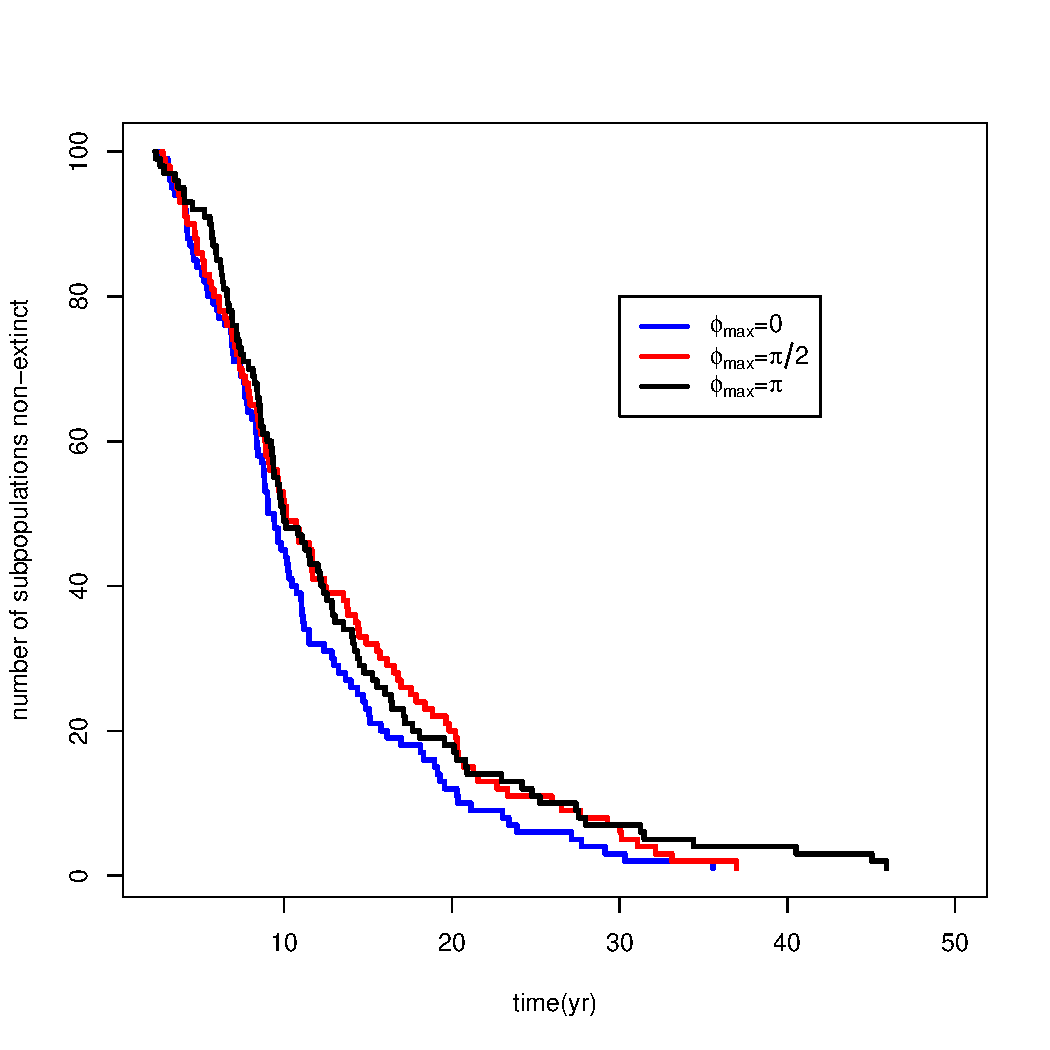
\includegraphics[scale=0.4]{smRep100Vil02R001N3e5} \protect\caption{Kaplan-Meier survival curves for disease persistence after 100 different
simulations of $\varphi_{max}=0$, $\varphi_{max}=\pi/2$ and $\varphi_{max}=\pi$.
The disease persistence time of $\varphi_{max}=0$ is the shortest
and that of $\varphi_{max}=\pi$ is the longest.}


\label{fig:persm100phi0pi2pi_01} 
\end{figure}


The phase of forcing of the $subpopulation_{1}$ is always fixed at
$0$, but that of the $subpopulation_{2}$ increases from $0$ to
$\pi$. In the first experience $\varphi_{max}=0$, the two subpopulations
are in synchrony with all beginning conditions. In the simulation
time, they are easy to find local extinctions together. The metapopulation
goes globally extinct in a short time. The disease persistence time
is the shortest. Moreover, the two subpopulations become asynchronous
when $\varphi_{max}=\pi/2$ or $\pi$. The symmetry of fixed points
is just broken at the starting moment. The level of synchrony of the
metapopulation decreases. The level of asynchrony $\varphi_{max}$
is directly scaled with the phase difference in the forcing rates,
but inversly with the global persistence time. When \textbf{$\varphi_{max}=\pi$,
}the two subpopulations are in antiphase. The balance points at the
begining moment of $subpopulaiton_{1}$ are inverse to that of $subpopulation_{2}$,
they accounts for why the two subpopulations take a long duration
to obtain the balance state. This is the most difficult case to find
global extinction, the persistence time is the longest. Moreover,
theses obtained results are also explicated by the recolonization
between the two subpopulations. When the disease no longer exists
in one subpopulation at the moment $t$. If at this moment, all neighbouring
subpopulations obtain also the extinction, so we have a global extinction
in the metapopulation and the disease is entirely extinct. However,
in a metapopulation, due to different factors for migration between
subpopulations, we hardly see extinction at the same time in all subpopulations
in first duration. The infected in other subpopulation migrates to
the extinct subpopulation, so the disease is active. It is the reason
why the disease exists for long term. In short, the level of synchrony
between subpopulation is stronger, metapopualtion is easier to find
global extinction. Make all subpopulations synchronize is the easiest
way at which disease goes to extinct.

Additionally, we have exploited experiences on local fluctuations
of subpopulations. Here, local fluctuations is called local dynamics
or local noises. This is an important factor that can increase local
extinction numbers but make global extinction rate reduce as the following
figure\textbf{ }\ref{figRELA_LocalEXT_nbSUBPOP_phiMAXprobVISIT01}.

\begin{figure}[tbph]
\centering 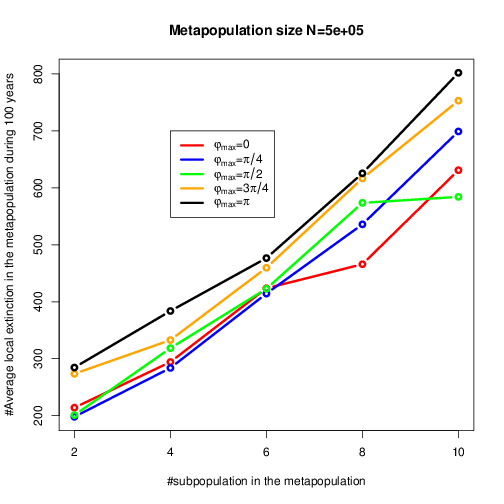
\includegraphics[scale=0.4]{figRELA_LocalEXT_nbSUBPOP_phiMAXprobVISIT01}
\protect\caption{Influence of the variation's asynchronic parameter on the relation
between the average number of local extinctions and the number of
subpopulations in a metapopulation. The number of iterations = 100
for each parameter; the probability of foreign visit=0.1; the metapopulation
size = 5e+05. }


\label{figRELA_LocalEXT_nbSUBPOP_phiMAXprobVISIT01}
\end{figure}


As the result shown in the figure \ref{figRELA_LocalEXT_nbSUBPOP_phiMAXprobVISIT01},
the rate of asynchrony $\varphi_{max}$ robustly affects the relation
between the average local extinction number and the number of subpopulation
in a metapopulation. We can find two main results here. First, the
average local extinction number in any metapopulation has an clear
increase when the rate of asynchrony $\varphi_{max}$ augments. At
the rate $\varphi_{max}=0.0$, it means to set the entire metapopulation
in the synchrony state, the dynamics of all subpopulations are synchronous
and the local extinction positions of the subpopulation may be also
synchronous. Therefore, this average number in the metapopulation
is minimum. Inversely, when the rate of asynchrony $\varphi_{max}$
starts tending to increase, the fluctuations are also changed and
fallen into the difference phase. It is the reason why when a subpopulation
goes locally extinct and after it is redominated in a short time by
disease due to the recolonisation among subpopulations. At the rate
$\varphi_{max}=\pi$, the difference phase is maximum. The average
number of local extinction in a metapopulation is maximum. Second,
in a metapopulation, if the subpopulation number increases, then the
local extinction number augments also. Because when the subpopulation
number is directly scaled with the metapopulation size and the time
of disease persistence. In addition, the interaction among subpopulation
increases with the subpopulation number. One subpopulation is easy
to be dominated by the other subpopulations due to the recolonisation.


\subsection{Quantifying global extinction rate and asynchrony level $\varphi_{max}$}

As mentioned about, we use survival regression model for global peristence
curve to estimate its global extinction rate for each value $\varphi_{max}$
with confidence interval 95\%. The result below is pointed for the
metapopulation of 15 subpopulations, the metapopulation size $N=10^{6}$
and the coupling rate $\rho=0.1$ as following figure \ref{fig:perrateVil15Rho01n1e6}.

\begin{figure}[tbph]
\centering 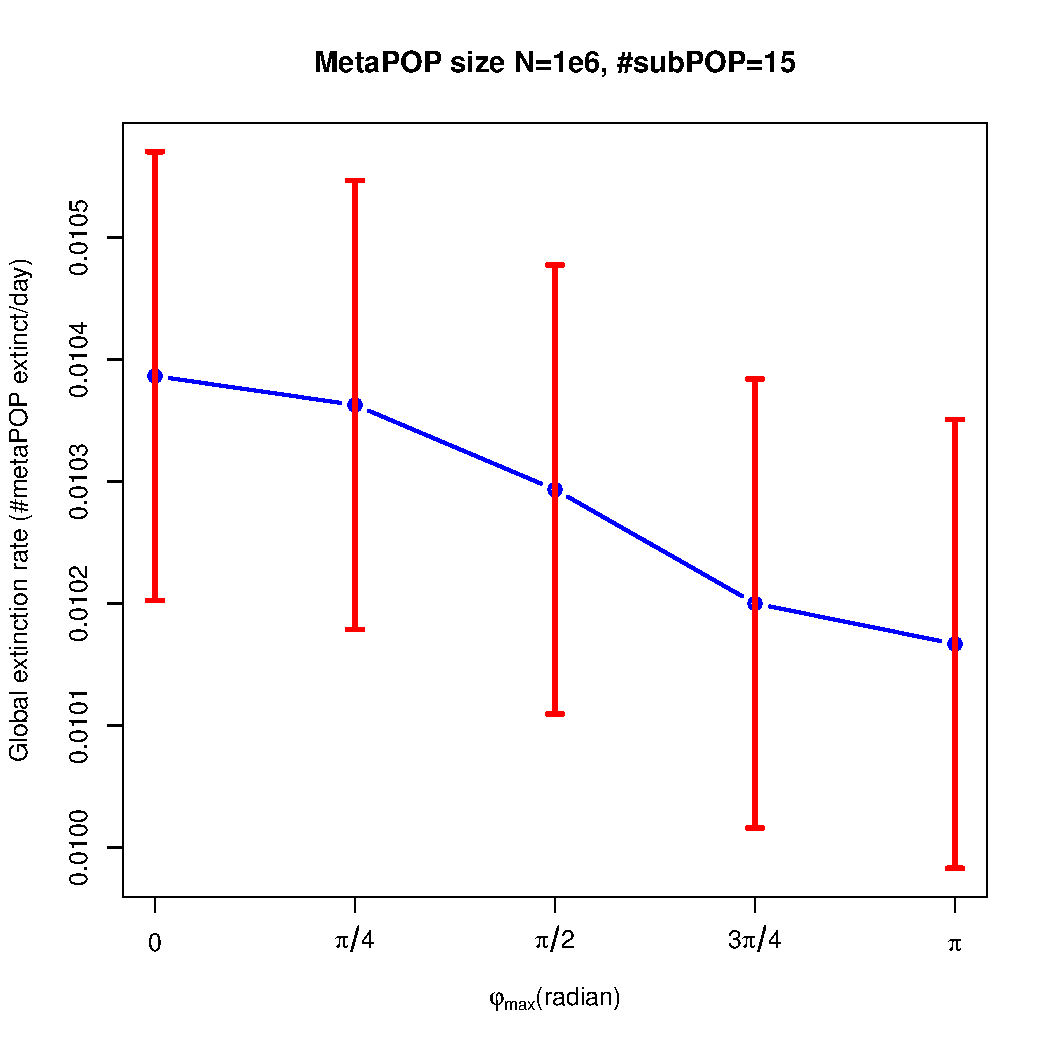
\includegraphics[scale=0.4]{plotIntvMeta15N1e6} \protect\caption{Estimated th global etinction rates in the metapopulation of the 15
subpopulations after 100 different simulations $N=10^{6}$, coupling
rate $\rho=0.1$. Here, with 95\% confidence interval, the red lines
and the red points are respectively the confidence intervals and the
estimated rates for the global extinction rate of each value of $\varphi_{max}$.}


\label{fig:perrateVil15Rho01n1e6} 
\end{figure}


This figure \ref{fig:perrateVil15Rho01n1e6} shows to us that the
amplitude of the confidence intervals for each value of $\varphi_{max}$
are quite far to each other. Furthermore, it goes down robustly when
$\varphi_{max}$ runs from $0$ to $\pi$. The phase difference strongly
influences the global disease extinction rate. Figure \ref{fig:perrateVil15Rho01n1e6}
indicates the trend of the extinction rate with decreasing the level
of asynchrony. The asynchrony between subpopulations is the main reason
why the infectious disease goes extinct in the slow way.


\subsection{Influence of other parameters on global extinction rate}


\subsubsection{Number of subpopulation in a metapopulation}

In this part, we developed the relation between the mass extinction
rate and the number of subpopulations in a metapopulation. We performed
simulations with metapopulations from two to 30 subpopulations, population
sizes of each subpopulation $N=5e+05$ and $\varphi_{max}=\pi/2$.
The result as following figure \ref{FigGlobExtNbVilles}.

\begin{figure}[tbph]
\centering 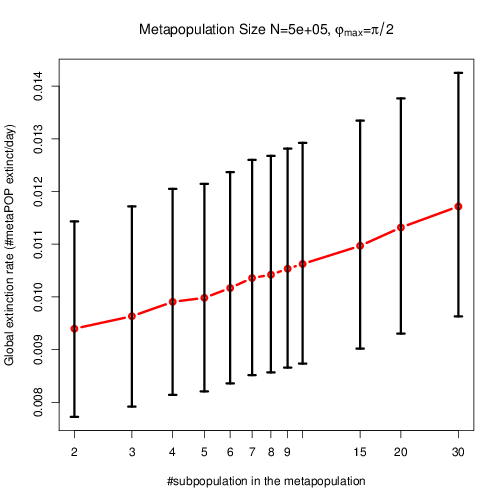
\includegraphics[scale=0.4]{plotTOTALnbvillesPhipi2}
\protect\caption{Estimated global extinction rates in different metapopulations after
100 different simulations with the metapopulation size fixed $N=5\times10^{5}$,
coupling rate $\rho=0.1$ and $\varphi_{max}=\pi/2$. Here, with 95\%
confidence interval, the black lines and the red points are respectively
the confidence intervals and the estimated rates for the global extinction
rate of each metapopulaion.}


\label{FigGlobExtNbVilles}
\end{figure}


The result (figure \ref{FigGlobExtNbVilles}) exhibits to us that
the number of subpopulations strongly has an influence for the disease
persistence time. The global extinction rate of an infectious disease
in a metapopulation increases when the number of subpopulations in
this metapopulation increases. With the metapopulation size is fixed,
when the number of cities in the metapopulation goes up, it means
that the population size of each subpopulation is declined. In particular,
the population size of each subpopulation is very small when the number
of cities reaches to 30. The dynamic in a small population goes fastly
extinct. Althought, the model used is the coupling metapopulations,
there are interactions among subpopulations and recolonisations of
desease. But because the population size is small, the number of visiteurs
going to other subpopulation is very little. The time of disease persistence
in a population having the small size is short. We fastly find the
mass extinction in the metapopulation. 


\subsubsection{Influence of the metapopulation size}

In the metapopulation of $05$ subpopulations, we implemented experiences
with different population sizes of subpopulation. We performed $100$
different simulations for the metapopulation of $05$ subpopulations
in which their sizes follow a stationary distribution of the metapopulation
size \textbf{$N$}. We set $N$ from $5\times10^{5}$ to $5\times10^{6}$
individuals. The result (Figure \ref{FigMetaSizeGlobExt}) affirms
that the size $N$ influences strongly the global persistence of an
infectious disease in a metapopulation.

\begin{figure}[tbph]
\centering 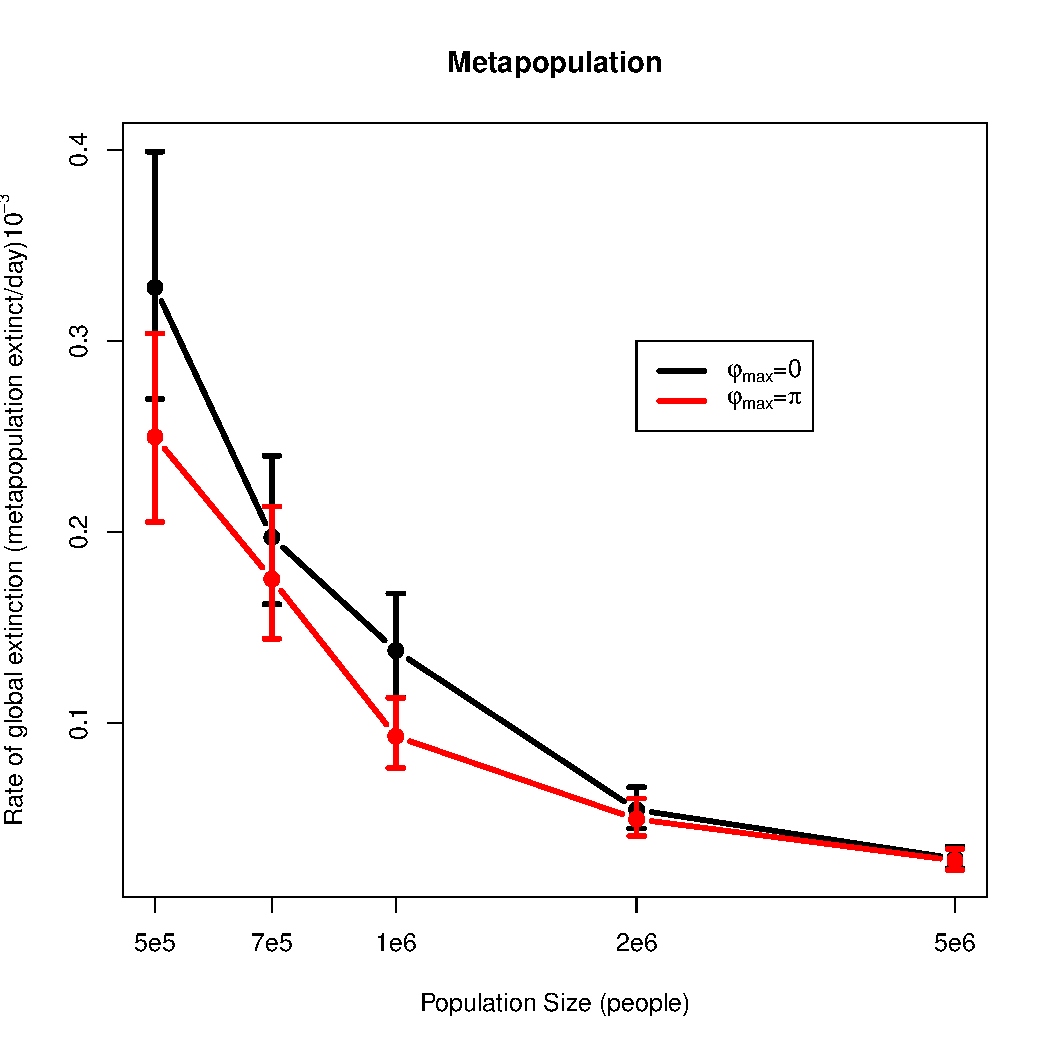
\includegraphics[scale=0.4]{resPOPSIZE_interval} \protect\caption{The relation between the metapopulation size and the global extinction
rate for the metapopulation of five subpopulations.}


\label{FigMetaSizeGlobExt}
\end{figure}


From the figure \ref{FigMetaSizeGlobExt}, we find that the mass extinction
rate goes down when the metapopulation size augments, at the same
time, these rates decreases when the asynchrony $\varphi_{max}$ goes
up. It is obvious that the metapopualtion size is big, then the time
of disease persistence augments, then the mass extinction rates is
declined..


\subsubsection{Coupling rate}

One more factor that was pointed is coupling strength between subpopulations.
Here, the coupling rate or the dispersal rate $\rho$ can be considered
as migration strength. The disease transmission speed grows fast when
coupling rate goes up in metapopulations, but the global extinction
rate is inverse (Figure \ref{fig:resPenteVil05multiRho-1}). In this
part, we change coupling rate from weak to strong in a metapopualtion
of five subpopulations with the metapopulation size $N=10^{6}$ .
The dispersal rate $\rho$ is divided into three intervals. These
are low, intermediate and high coupling rate intervals. In each interval,
we chose some coupling rates that highlight the coupling strength
among subpopulations in a metapopulation. When the coupling rate is
small from $0.0$ to $0.005$, the mass extinction rate decreases
very slowly. Because, in this case, the subpopulations seem to be
independent. They fluctuate independently. They are easy to go extinct.
We are also easy to find the mass extinction in the metapopulation.
However, this extinction rate is declined in a sudden way when the
coupling rate is modified from $0.01$ to $0.3$. Lastly, the extinction
rate increases when the coupling rate is so robust from $0.5$ to
$1.0$. Based on this figure, the mass extinction rate in a metapopulation
is one inverse bell for the coupling rate. The medium coupling rate
(from $0.01$ to $0.1$) minimizes the mass extinction rate in metapopulation.
As in the case of the small and average coupling rates, the coupling
rate and the speed of migration among subpopulations are directly
proportional. The dispersal speed increases, thereby the local recolonization
speed rises, the duration of persistence grows. However, this trend
of global extinction rate with decreasing coupling rate, is not right
any more when the dispersal rate is strong. The duration of persistence
falls, because the metapopulation has tendency to become one big population.
In this case, the phase difference or the recolonization among subpopulations
are no longer significant.

\begin{figure}[tbph]
\centering 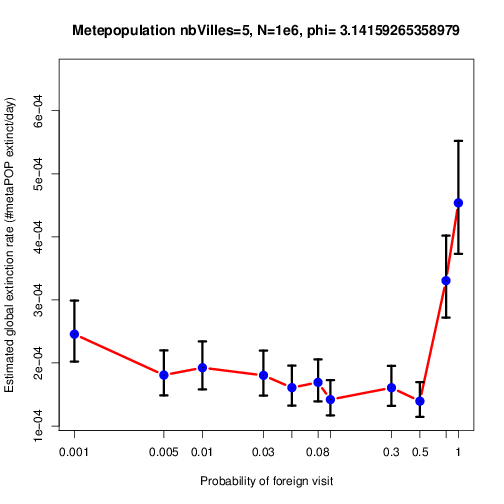
\includegraphics[scale=0.4]{plotprobVISITERVIl5N1e6PHIMAXpi_EXT}
\protect\caption{Correlation between the coupling rate and the mass extinction rate
in the metapopulation of five subpopulations. Here, the coupling rate
$\rho$ runs from 0 to 1. The level of asynchrony $\varphi_{max}$
is $\pi$ and the metapopulation size N=1e6.}


\label{fig:resPenteVil05multiRho-1} 
\end{figure}



\section{Discussion and Conclusion}

We successfully have built a version for the susceptible-infectied-recovered
stochastic metapopulation model. The infection rate $\lambda_{i}$
for \textbf{$subpopulation_{i}$ }has portrayed all effects inside
as well as outside of the disease tranmission chain between individuals
in the same subpopulation or in other subpopulations. Moreover\textbf{,
}our metapopulation model became more detailed when we brought seasonality\textbf{
}in metapopulation model to create periodic transmission in year that
highlighted seasonal changes as well as school period of children
\cite{Bolker1993,Bolker1995,Earn1998,Keeling2002}\textbf{. }We have
metapopulation model with different contact rates for each subpopulation.
This is a more complex model than any used metapopulation model. We
have sketched successfully in-phase and sometime out-of-phase (``antiphase'')
models across suburbs of He's 2003 \cite{He2003}

This complex metapopulation model is also an expected result of Rozhnova(2012)
\cite{Rozhnova2012}. It's a good result for scientists wanting to
use the SEIR metapopulation model for simulating dynamics of infectious
diseases. Our results roughly support those of Rozhnova's 2012. The
authors gave different values of the contact rates $\beta$ of each
subpopulation. However, the rates $\beta$ here are fixed by constants
and the number of subpopulations in experiences are maximum of three.
Comparing this result with our's, in a coupling metapopulation, the
degree of synchorny is maintained when the coupling rate between subpopulations
is weak.

Moreover, our stochastic SEIR metapopulation model with subpopulations
connected to each other, we have quantified disease persistence of
seasonality as well as spatial synchrony. With our model, we can easily
create level of seasonality in year and at the same time, phase difference
in seasonality between subpopulations. It's the reason why we have
model quite close to the metapopulation model in reality.

Due to the phase difference between the number of contact $\kappa$,
we can change by an increase or a decrease in level of synchrony.
We want to decrease level of synchrony, by simply increasing the phase
difference between forcing phase coefficients in the formulas of the
number of contact $\kappa$. Clearly, the level of synchrony between
two subpopulations are the worst when the two fluctuations are in
antiphase (as figure \ref{fig:persm100phi0pi2pi_01}). When the phase
difference between oscillations increases, the desynchronizing effect
on population dynamics of the subpopulations augments. This enhances
disease persistence time though the global extinction rate is reduced.
Moreover, as the result above (figure \ref{fig:perrateVil15Rho01n1e6}),
in the local shape,\textbf{ }our result, along with those of Bolker
(1995) \cite{Bolker1995} and Heino (1997) \cite{Heino1997}, stress
the number of local extinctions\textbf{ }being inversely proportionnel
with the global extinction rate in a metapopulation. When the level
of synchrony is at a reduction and the global persistence time gets
an increase, the global extinction rate of metapopulation goes down
and the number of local extinction goes up. Due to the result about
local extinction, we also affirm that disease is always available
in metapopulation if and only if at least one subpopulaiton is not
extinct.\textbf{ }

Our finding has specified the two main factors influencing the persistence
ability of an infectious disease. One factor is transmission characteristics
of the infectious disease and the other is interplay between mixing
subpopulations in metapopulation. The interaction between the disease
persistence and the spatial heterogeneity becomes a major key to unlock
questions about infectious disease in epidemiology. This result takes
a large part in epidemic disease persistence domain that has being
exploited in scientific epidemically research works. We gained a robust
understanding of how disease persistence is affected by local factors
such as spatial heterogeneity, demographic asynchrony and seasonality,
as well as mixing factors such as migration, disease transmission
between hosts and pathogens. Lastly, we also highlighted recolonization
effects. It is like rescue for disease. Because of connection between
subpopulation, individuals can go everywhere. Subpopulation is quickly
re-infected althought the disease has became extinct. Thus, the disease
rescus makes local extintions difficult to extend into global extinctions.

As a matter of the fact of coupling strength among subpopulations
in metapopulation, we proved that the curve of the global extinction
rate is a convex function following the coupling rate. Inversely,
the persistence of the disease in the metapopulation is an exponential
survival function over time and is a humped function for the coupling
rate. In addition, when the coupling rate between subpopulations is
just medium where the mass extinction rate is minimum and the global
disease persistence in metapopulation is maximum . This finding is
similar to those of Huffaker(1958) \cite{huffaker1958experimental},
Holyoak and Lawler(1996) \cite{holyoak1996persistence}, and Yaari
et al. (2012) \cite{Yaari2012} when they exhaustively explored the
disease persistence behavior of many different metapopulation models.
And our result one more time affirms that the interaction in metapopulation
models plays a big role when\textbf{ }the interaction strength $\rho$
is from $10^{-3}$ to $0.1$ \cite{KeelingRohani2008}.

To summarize, we have built successfully a\textbf{ }sinusoidally forced
SEIR stochastic metapopulation model. This model is like a physical
system of coupled oscillators. We have pointed out that spatial synchronization
consistently and predictably makes extinction risk increase by using
the model $0$ where all the subpopulations have the same population
size $N$ and there is no explicit spatial distance. So, it's good
for the future, we can continue this work with different population
size of each subpopulation and different spatial distance between
subpopulations and then, create synchronous metapopulations that optimize
vaccination policies.

\bibliographystyle{plain}
\bibliography{bikBokEpidemics,bikCCS,bikPerSyns,bibStateDisease}


\newpage{}


\section{Appendix : equilibrium values of the system \ref{eq:dS}--\ref{eq:dR}}

We start with ordinary differential equations for a $subpopulation_{i}$
in a metapopulation as follows:

\begin{eqnarray}
\frac{dS_{i}}{dt} & = & \mu N_{i}-\lambda_{i}S_{i}-\mu S_{i}\\
\frac{dE_{i}}{dt} & = & \lambda_{i}S_{i}-\mu E_{i}-\sigma E_{i}\\
\frac{dI_{i}}{dt} & = & \sigma E_{i}-\mu I_{i}-\gamma I_{i}\\
\frac{dR_{i}}{dt} & = & \gamma I_{i}-\mu R_{i}
\end{eqnarray}
 In simulation, we know that the equilibrium state allow a disease
to persist in a population for a long time. So, an infectious disease
in the $subpopulation_{i}$ is available in long term this system
is at equilibrium. It means that at which $\frac{dS_{i}}{dt}=\frac{dE_{i}}{dt}=\frac{dI{}_{i}}{dt}=\frac{dR{}_{i}}{dt}=0$
({*}). Thus, we let all equations (equations $15$ - $18$ ) in the
system be equal to zero, then calculate the values of the variables
(now denoted by $S_{i}^{*}$, $E_{i}^{*}$, $I_{i}^{*}$ , and $R{}_{i}^{*}$)
that satisfy this condition ({*}). We have these values as folllows:

\begin{eqnarray}
S_{i}^{*} & = & N_{i}\frac{(\gamma+\mu)(\sigma+\mu)}{\beta\sigma}\\
E_{i}^{*} & = & N_{i}\mu\left(\frac{1}{\sigma+\mu}-\frac{\gamma+\mu}{\beta\sigma}\right)\\
I_{i}^{*} & = & N_{i}\mu\frac{\beta\sigma-(\sigma+\mu)(\gamma+\mu)}{\beta(\sigma+\mu)(\gamma+\mu)}\\
R_{i}^{*} & = & N_{i}-S_{i}^{*}-E_{i}^{*}-I_{i}^{*}
\end{eqnarray}


Here, if we set $R_{0}=\frac{\beta\sigma}{(\gamma+\mu)(\sigma+\mu)}$,
so we have

\begin{eqnarray}
S_{i}^{*} & = & N_{i}\frac{1}{R_{0}}\\
E_{i}^{*} & = & N_{i}\frac{\mu\sigma}{R_{0}}\left(R_{0}-1\right)\\
I_{i}^{*} & = & N_{i}\frac{\mu}{\beta}(R_{0}-1)\\
R_{i}^{*} & = & N_{i}-S_{i}^{*}-E_{i}^{*}-I_{i}^{*}
\end{eqnarray}


One nomal conditions for all population availabes is that the equilibrium
values cannot be negative. Therefore, an infectious disease is available
in the $subpopulation_{i}$ if $R_{0}>1$. Now, the endemic equilibrium
in the system is given by $(S_{i}^{*},E_{i}^{*},I{}_{i}^{*},R{}_{i}^{*})$
= $(N_{i}\frac{1}{R_{0}}$, $N_{i}\frac{\mu\sigma}{R_{0}}\left(R_{0}-1\right)$,
$N_{i}\frac{\mu}{\beta}(R_{0}-1)$, $N_{i}(1-\frac{1}{R_{0}}-\frac{\mu\sigma}{R_{0}}\left(R_{0}-1\right)-\frac{\mu}{\beta}(R_{0}-1))$.\newpage{}


\section{Appendix: derivation of the equation \ref{eq:force-1}}

Here, we will point out that the contact rate $\beta$ is a function
of the average contact number per unit of time and the probability
of successful disease transmission following a contact.
\begin{defn}
During the small time interval $\delta t$, each individual native
of the subpopulation $i$ visits one single subpopulation\textbf{
}$j$ (with the probability $\rho_{ij}$) and will see in average
$\kappa_{j}$ individuals. These individuals come from all the cities.
\end{defn}

\subsection{Notation :}

Here, we present list of sets and events describing the state of the
system at time $t$ : 
\begin{itemize}
\item $C_{i}$ is the set of all individuals born in subpopulation $i$. 
\item $V_{i,t}$ is the set of all individuals physically located in subpopulation
$i$ from time $t$ to time $t+\delta t$. This includes foreigners
traveling in subpopulation $i$ at time $t$, and all natives from
subpopulation $i$ which are not traveling abroad at time $t$. 
\item $S_{t},E_{t},I_{t},R_{t}$ are the sets of all individuals respectively
susceptible, exposed, infected and recovered at time $t$. Note that
these set include individuals from all subpopulations. 
\item $S_{i,t},E_{i,t},I_{i,t},R_{i,t}$ are the same sets, restricted to
natives of subpopulation $i$. So formally, $S_{i,t}=S_{t}\cap C_{i}$,
$E_{i,t}=E_{t}\cap C_{i}$, $I_{i,t}=I_{t}\cap C_{i}$, and $R_{i,t}=R_{t}\cap C_{i}$. 
\item $Transmit(y,x)$ is an event indicating that individual $x$ gets
infected by individual $y$ which was already infected 
\item $c_{i,k}$ is the probability that a susceptible individual native
from $i$ being in contact with another infected individual native
from $k$ gets infected. 
\item $\kappa_{j}$ is the average number of contacts per unit of time a
susceptible will have when visiting subpopulation $j$. 
\item $\xi_{jk}$ refers to the probability that an individual $y$ meeting
$x$ in $C_{j}$ comes from $C_{k}$.
\item $\rho_{i,j}$, the probability that an individual from subpopulation
$i$ visits subpopulation $j$. Of course, $\sum_{j=1}^{M}\rho_{ij}=1$.\end{itemize}
\begin{prop}
The coefficient $\kappa$ should also depend on $i$, because an individual
native from subpopulation $i$ meets more people in his own subpopulation
than abroad ($\kappa_{i,i}>\kappa_{i,j}$). 
\end{prop}

\subsection{The background}

One general question is always posed ``how does the population of
exposed individuals of subpopulation $i$ evolve ?''. For the sake
of simplicity, in the process of transmission of the SEIR model, we
focus on the incidence and we assume for now that the latent period
and the recovery rate, repectively $\mu=\sigma=0$. Thus, we write
a probabilistic formulation of $\frac{dE_{i}}{dt}$. Assuming the
time is discrete, we have $\frac{dE_{i}}{dt}\approx\mathbb{E}\left[E_{i,t+1}\setminus E_{i,t}\right]$.
Then,

\begin{eqnarray*}
\mathbb{E}\left[E_{i,t+1}\setminus E_{i,t}\right] & = & \mathbb{E}\left[E_{i,t+1}\cap S_{i,t}\right]\\
 & = & \sum_{x\in C_{i}}Pr\left[x\in E_{t+1}\wedge x\in S_{t}\right]\\
 & = & \sum_{x\in C_{i}}Pr\left[x\in S_{t}\right]*Pr\left[x\in E_{t+1}\mid x\in S_{t}\right]\\
 & = & Pr_{x\sim\mathcal{X}_{i}}\left[x\in E_{t+1}\mid x\in S_{t}\right]*\sum_{x\in C_{i}}Pr\left[x\in S_{t}\right]\\
 & = & |S_{i,t}|\times Pr_{x\sim\mathcal{X}_{i}}\left[x\in E_{t+1}\mid x\in S_{t}\right]
\end{eqnarray*}


Assume there are $M$ cities. An individual $x$ of the subpopulation
$i$ may be visiting another subpopulation, or staying in its own
subpopulation. Applying the law of total probabilities, we get:

\begin{eqnarray*}
Pr_{x\sim\mathcal{X}_{i}}\left[x\in E_{t+dt}\mid x\in S_{t}\right] & = & \sum_{j=1}^{M}Pr_{x\sim\mathcal{X}_{i}}\left[x\in E_{t+dt}\wedge x\in V_{j,t}\mid x\in S_{t}\right]\\
 & = & \sum_{j=1}^{M}Pr_{x\sim\mathcal{X}_{i}}\left[x\in E_{t+dt}\mid x\in S_{t}\wedge x\in V_{j,t}\right].Pr_{x\sim\mathcal{X}_{i}}\left[x\in V_{j,t}\right]\\
 &  & \sum_{j=1}^{M}Pr_{x\sim\mathcal{X}_{i}}\left[x\in E_{t+dt}\mid x\in S_{t}\wedge x\in V_{j,t}\right]\times\rho_{ij}
\end{eqnarray*}


Where $\rho_{i,j}=Pr_{x\sim\mathcal{X}_{i}}\left[x\in V_{j,t}\right]$,
the probability that an individual from subpopulation $i$ visits
subpopulation $j$. Of course, $\sum_{j=1}^{M}\rho_{ij}=1$.


\subsection{Study of case where agent $x$ native from subpopulation $i$ visits
subpopulation $j$}

Here, we look at the probability that a susceptible $x\sim\mathcal{X}_{i}$
visiting $j$ gets infected or not after $\delta t$ time steps. Let
$\mathcal{Y}$ be the uniform distribution over $V_{j,t}$. The correct
mathematical approach for this would be to assume that for each subpopulation
$k$, the number of people native from $k$ that we meet during $\delta t$
follows a Poisson process. So both the number of people we meet and
the number of infected people we meet during $\delta t$ should be
random variables.

In the approach described in \cite{KeelingRohani2008}, the authors
did not do this. They assumed that both the number of people we meet
and the number of infected people we meet \emph{are fixed} (otherwise
the maths they write would have been different). We will call this
the ``Keeling \& Rohani'' interpretation that we will present it
in the following parts.

We introduce an alternative approximation, where we assume that the
number $\kappa$ of people we meet during $\delta t$ is \emph{fixed},
but each of these people has \emph{some probability} to be infected.
This is an \emph{in-between interpretation}, easier than the Poisson
process maths, but better than Keeling\&Rohani's one. We will call
this the ``Yann-Giang'' interpretation.


\subsubsection{The ``Yann-Giang'' interpretation}
\begin{prop}
Agent $x$ meets \emph{exactly} $\kappa_{j}$ other individuals, and
each of these individuals has a probability $\frac{\left|I_{k,t}\right|}{N_{k}}$
of being infected, where $k$ is its native subpopulation. Let $y_{1}\ldots y_{\kappa_{j}}$
be the individuals that $x$ meets. We get:
\end{prop}
\begin{eqnarray*}
 &  & Pr_{x\sim\mathcal{X}_{i}}\left[x\in S_{t+\delta t}\mid x\in S_{t}\wedge x\in V_{j,t}\right]\\
 & = & Pr_{x\sim\mathcal{X}_{i},y_{1}\ldots,y_{\kappa_{j}}\sim\mathcal{Y}}\left[\bigwedge_{p=1}^{\kappa_{j}}\neg\left(y_{p}\in I_{t}\wedge Transmit(y_{p},x)\right)\mid x\in S_{t}\wedge x\in V_{j,t}\right]
\end{eqnarray*}


So we have:

\begin{eqnarray*}
 &  & Pr_{x\sim\mathcal{X}_{i}}\left[x\in S_{t+\delta t}\mid x\in S_{t}\wedge x\in V_{j,t}\right]\\
 & = & Pr_{x\sim\mathcal{X}_{i},y\sim\mathcal{Y}}\left[\neg\left(y\in I_{t}\wedge Transmit(y,x)\right)\mid x\in S_{t}\wedge x\in V_{j,t}\right]^{\kappa_{j}\delta t}
\end{eqnarray*}


Moreover, we have:
\begin{itemize}
\item the probability so that a susceptible individual $x$ is infected
by an infected individual $y$ :
\end{itemize}
\begin{eqnarray*}
 &  & Pr_{x\sim\mathcal{X}_{i},y\sim\mathcal{Y}}\left[y\in I_{t}\wedge Transmit(y,x)\mid x\in S_{t}\wedge x\in V_{j,t}\right]\\
 & = & \sum_{k=1}^{M}Pr_{x\sim\mathcal{X}_{i},y\sim\mathcal{Y}}\left[y\in I_{t}\wedge Transmit(y,x)\mid x\in S_{t}\wedge x\in V_{j,t}\wedge y\in C_{k}\right].Pr_{y\sim\mathcal{Y}}\left(y\in C_{k}\right)\\
 & = & \sum_{k=1}^{M}\left\{ Pr_{x\sim\mathcal{X}_{i},y\sim\mathcal{X}_{k}}\left[y\in I_{t}\mid x\in S_{t}\wedge x\in V_{j,t}\right]\right.\\
 &  & \,\,\,\,\,\left.\times Pr_{x\sim\mathcal{X}_{i},y\sim\mathcal{X}_{k}}\left[Transmit(y,x)\mid y\in I_{t}\wedge x\in S_{t}\wedge x\in V_{j,t}\wedge y\in C_{k}\right]\times Pr_{y\sim\mathcal{Y}}\left(y\in C_{k}\right)\right\} \\
 & = & \sum_{k=1}^{M}\left(\frac{\left|I_{k,t}\right|}{N_{k}}\times c_{ik}\times\xi_{jk}\right)
\end{eqnarray*}


$\xi_{jk}=\frac{N_{k}\rho_{kj}}{\sum_{v=1}^{M}N_{v}\rho_{vj}}$ refers
to the probability that an individual $y$ meeting $x$ in $C_{j}$
comes from $C_{k}$.
\begin{itemize}
\item hence, the probability so that a susceptible individual $x$ is not
infected by an infected individual $y$ :
\end{itemize}
\[
1-\sum_{k=1}^{M}\left(\frac{\left|I_{k,t}\right|}{N_{k}}\times c_{ik}\times\xi_{jk}\right)
\]

\begin{itemize}
\item thereby, the probability so that a susceptible individual $x$ is
not infected after $\kappa_{j}$ contacts per unit time $\delta t$.
\end{itemize}
\[
\left[1-\sum_{k=1}^{M}\left(\frac{\left|I_{k,t}\right|}{N_{k}}\times c_{ik}\times\xi_{jk}\right)\right]^{\kappa_{j}\delta t}
\]

\begin{itemize}
\item thus, the probability so that a susceptible individual $x$ becomes
infected after $\kappa_{j}$ contacts per unit time $\delta t$.
\end{itemize}
\begin{eqnarray*}
Pr_{x\sim\mathcal{X}_{i}}\left[x\in E_{t+\delta t}\mid x\in S_{t}\wedge x\in V_{j,t}\right] & = & \left[1-\sum_{k=1}^{M}\left(\frac{\left|I_{k,t}\right|}{N_{k}}\times c_{ik}\times\xi_{jk}\right)\right]^{\kappa_{j}\delta t}
\end{eqnarray*}


We now apply the \emph{log} approximation which consists in approximating
$1-(1-u)^{v}$ by $v\log(1-u)$:

\begin{eqnarray*}
Pr_{x\sim\mathcal{X}_{i}}\left[x\in E_{t+\delta t}\mid x\in S_{t}\wedge x\in V_{j,t}\right] & = & -\kappa_{j}\delta t\log\left[1-\sum_{k=1}^{M}\left(\frac{\left|I_{k,t}\right|}{N_{k}}\times c_{ik}\times\xi_{jk}\right)\right]
\end{eqnarray*}


So, the transmission rate per susceptible individual is as follows
:

\[
\frac{dPr_{x\sim\mathcal{X}_{i}}\left[x\in E_{t+dt}\mid x\in S_{t}\wedge x\in V_{j,t}\right]}{dt}\simeq-\kappa_{j}\log\left[1-\sum_{k=1}^{M}\left(\frac{\left|I_{k,t}\right|}{N_{k}}\times c_{ik}\times\xi_{jk}\right)\right]
\]


In fact, we use the parameter $\lambda$ to present this quantity,
and it is denoted as the ``force of infection'' :

\[
\lambda_{i}=\sum_{j}\rho_{ij}\kappa_{j}\log\left[1-\sum_{k=1}^{M}\left(\frac{\left|I_{k,t}\right|}{N_{k}}\times c_{ik}\times\xi_{jk}\right)\right]
\]


If there is only one subpopulation $i$, then

\[
\lambda_{i}=\kappa_{j}log(1-\frac{\left|I_{i}\right|}{N_{i}}\times c_{ii})
\]



\subsubsection{``Keeling \& Rohani'' Interpretation}
\begin{prop}
Agent $x$ meets \emph{exactly} $\kappa_{j}\delta t\xi_{jk}\frac{\left|I_{k,t}\right|}{N_{k}}$
other infected individuals native from subpopulation $k$.

Let $l_{k}=\kappa_{j}\delta t\xi_{jk}\frac{\left|I_{k,t}\right|}{N_{k}}$. 


Let $y_{1}^{k}\ldots y_{l_{k}}^{k}$ be the infected individuals native
from $k$ that our individual $x$ meets between $t$ and $t+\delta t$.

\end{prop}
We have the probability so that a susceptible individual $x$ is not
infected after having seen $l_{k}$ individuals between $t$ and $t+\delta t$
:

\begin{eqnarray*}
 &  & Pr_{x\sim\mathcal{X}_{i}}\left[x\in S_{t+\delta t}\mid x\in S_{t}\wedge x\in V_{j,t}\right]\\
 & = & Pr_{x\sim\mathcal{X}_{i}}\left[\bigwedge_{\begin{array}{c}
k=1\ldots M\\
p=1\ldots l_{k}
\end{array}}\neg\left(Transmit(y_{p}^{k},x)\right)\mid x\in S_{t}\wedge x\in V_{j,t}\right]\\
 & = & \prod_{k=1}^{M}Pr_{x\sim\mathcal{X}_{i}}\left[\bigwedge_{p=1\ldots l_{k}}\neg\left(Transmit(y_{p}^{k},x)\right)\mid x\in S_{t}\wedge x\in V_{j,t}\right]\\
 & = & \prod_{k=1}^{M}\left(1-c_{ik}\right)^{\kappa_{j}\delta t\xi_{jk}\frac{\left|I_{k,t}\right|}{N_{k}}}
\end{eqnarray*}


Then, we plug this back into the previous formula, and we get:

\begin{eqnarray*}
Pr_{x\sim\mathcal{X}_{i}}\left[x\in E_{t+\delta t}\mid x\in S_{t}\wedge x\in V_{j,t}\right] & = & 1-\prod_{k=1}^{M}\left(1-c_{ik}\right)^{\kappa_{j}\xi_{jk}\frac{\left|I_{k,t}\right|}{N_{k}}\delta t}
\end{eqnarray*}


The first order approximation of $1-\prod_{k=1}^{M}(1-c_{ik})^{v_{k}}$
is $\sum_{k=1}^{M}-v_{k}\log(1-c_{ik})$. Applying this approximation
here, we get:

\begin{eqnarray*}
Pr_{x\sim\mathcal{X}_{i}}\left[x\in E_{t+\delta t}\mid x\in S_{t}\wedge x\in V_{j,t}\right] & \simeq & \delta t\sum_{k=1}^{M}\left(-\kappa_{j}\xi_{jk}\frac{\left|I_{k,t}\right|}{N_{k}}\log\left(1-c_{ik}\right)\right)
\end{eqnarray*}


Define $\beta_{ijk}=-\kappa_{j}\log\left(1-c_{ik}\right)$, let $\delta t$
converge to zero, and we get:

\[
\frac{dPr_{x\sim\mathcal{X}_{i}}\left[x\in E_{t+dt}\mid x\in S_{t}\wedge x\in V_{j,t}\right]}{dt}\simeq\sum_{k=1}^{M}\left(\xi_{jk}\frac{\left|I_{k,t}\right|}{N_{k}}\beta_{ijk}\right)
\]


If there is only one subpopulation $i$, then we fall back to the
formula of \cite{KeelingRohani2008}. We have : 

\[
\beta_{i}=-\kappa_{i}\log\left(1-c_{i}\right)
\]


\[
\frac{d}{dt}\mathbb{E}\left[\left|E_{i,t+dt}-E_{i,t}\right|\right]\simeq-\left|S_{i,t}\right|\left(\frac{\left|I_{i}\right|}{N_{i}}\beta_{i}\right)
\]


and the force of infection as follows :

\[
\lambda_{i}=\beta_{i}\frac{\left|I_{i}\right|}{N_{i}}
\]



\subsection{Final Formula}

We simply have to plug in the probability $\rho_{ij}$ that $i$ visits
$j$.

We get, for the ``Yann-Giang'' interpretation :

\[
\frac{d}{dt}\mathbb{E}\left[\left|E_{i,t+dt}-E_{i,t}\right|\right]\simeq-\left|S_{i,t}\right|\sum_{j}\rho_{ij}\kappa_{j}\log\left[1-\sum_{k=1}^{M}\left(\frac{\left|I_{k,t}\right|}{N_{k}}\times c_{ik}\times\xi_{jk}\right)\right]
\]


And for the ``Keeling \& Rohani'' Interpretation :

\[
\frac{d}{dt}\mathbb{E}\left[\left|E_{i,t+dt}-E_{i,t}\right|\right]\simeq-\left|S_{i,t}\right|\sum_{j}\rho_{ij}\sum_{k=1}^{M}\left(\xi_{jk}\frac{\left|I_{k,t}\right|}{N_{k}}\beta_{ijk}\right)
\]


\newpage{}


\section*{Appendix: supplementary materials}


\section*{Relation between the average local extinction number and the number
of subpopulation in a metapopulation when the metapopulation size
varies:}

\begin{figure}
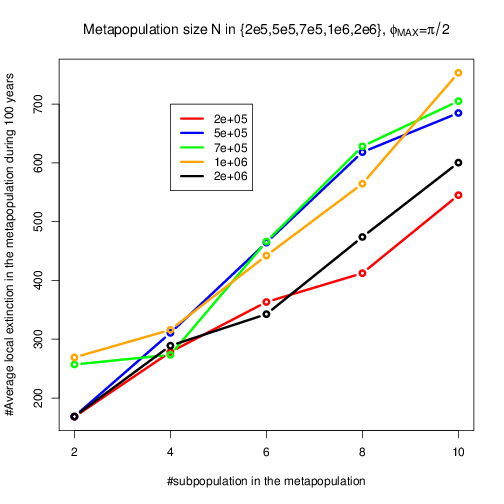
\includegraphics[scale=0.4]{/home/tran/Desktop/Réunion/figRELLocalEXTSubPOP_METASIZE_phiMAXpi2}\protect\caption{Influence of the variation of metapopulation size $N$ on the relation
between the average local extinction number and the number of subpopulation
in a metapopulation. }


\label{figRELLocalEXTSubPOP_METASIZE_phiMAX}
\end{figure}


The figure \ref{figRELLocalEXTSubPOP_METASIZE_phiMAX} shows the relation
between the average local extinction number and the number of subpopulation
in a metapopulation. We find that the local extinction number is minimum
when the metapopulation size is maximum. Because with a big metapopulation,
the size of a subpopulation is great. It is the reason why this subpopulation
is very difficile to find the local extinction. Inversely, when the
metapopulation size is small, then the persistence time is short.
Thus, this metapopulation goes to the global extinction in the easy
way. On the other hand, we can find that the metapopulation size in
the interval from $5e+05$ to $1e+06$, the local extinction number
is high. It means that the size of a subpopulation is approximately
from $1e+05$ to $5e+05$. This is the interval that permit a disease
to spread and permit the time of disease persistence to be enough
long to study. Finally, we get also the same result, the local extinction
number are in increase with the number of subpopulation in a metapopulation.


\section*{Relation between the average local extinction number and the number
of subpopulation in a metapopulation when the coupling rate varies:}

\begin{figure}
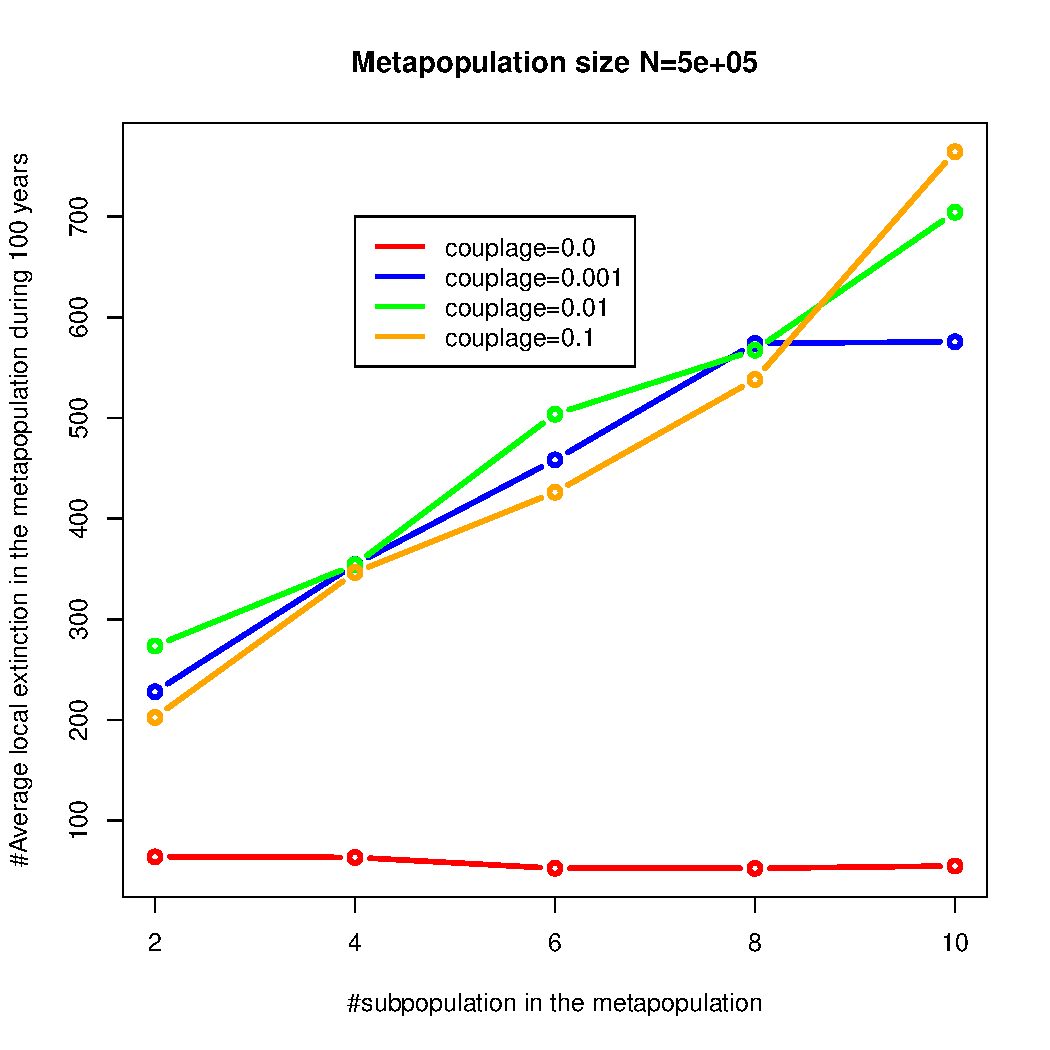
\includegraphics[scale=0.4]{/home/tran/Desktop/Réunion/figRELALocalEXTnbSUBPOPphiPI_couplage}

\label{figRELALocalEXTnbSUBPOPphiPI_couplage}

\protect\caption{Influence of the variation of coupling rate on the relation between
the average local extinction number and the number of subpopulation
in a metapopulation. }
\end{figure}


The results are found in the figure \ref{figRELALocalEXTnbSUBPOPphiPI_couplage},
the local extinction number is minimum when the coupling rate is equal
$0.0$. It is obvious that in a metapopulation where the subpopulations
are isolated, there is no recolonisation among subpopulation. After
the local extinction number strongly increases when the coupling rate
augments. However, this number is biggest when the coupling rate $\rho=0.01$.
Because at this rate where the subpopulations are in the mediate interaction.
Moreover the coupling rate and the speed of migration among subpopulations
are directly proportional. The dispersal speed increases, thereby
the local recolonization speed rises, the duration of persistence
grows. However, when the dispersal rate is more big, this trend of
local extinction number decreases. Because the metapopulation has
tendency to become one big population, so the phase difference or
the recolonization among subpopulations are no longer significant.
The following figure \ref{figLocalEXTCouplageSUBPOP4} is an other
resultat for the influence of the coupling rate on the local extinction
number in the metapopulation.

\begin{figure}
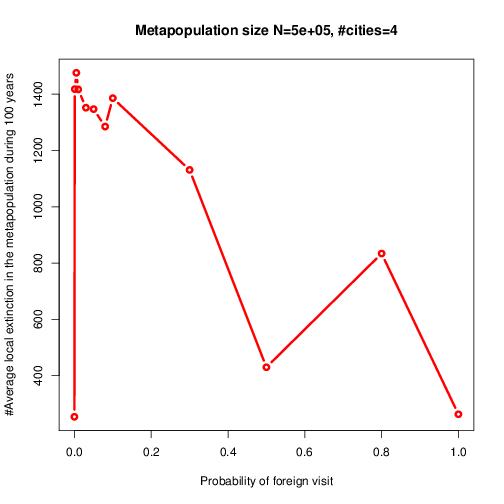
\includegraphics[scale=0.4]{/home/tran/Desktop/Réunion/figLocalEXTCouplageSUBPOP4}

\label{figLocalEXTCouplageSUBPOP4}

\protect\caption{Relation between the average local extinction number and the coupling
rate in the metapopulation of four subpopulations with the metapopulation
size $N=5e5$ and $\varphi_{max}=\pi$. }
\end{figure}

\end{document}
